\clearpage
\chapter{Orchestration Workflow}
\label{chp:Workflow}

The previous chapter has provided a detailed discussion on a number of task-specific languages, each one addressing an individual model management task. However, in practice, model management tasks are seldom carried out in isolation; instead, they are often combined together to form complex workflows. Therefore, of similar importance to the existence of individual task-specific management languages is the provision of a mechanism that enables developers to compose modular and reusable tasks into complex automated processes. In a broader context, to facilitate implementation of seamless workflows, an appropriate MDE workflow mechanism should also support mainstream development tasks such as file management, version control management, source code compilation and invocation of external programs and services.

\section{Motivation}
\label{sec:Workflow.Motivation}

As a motivating example, an exemplar workflow that consists of both MDD tasks (1-4, 6) and mainstream software development tasks (5, 7) is displayed below.

\begin{enumerate}
	\item Load a UML model
	\item Validate it
	\item Transform it into a Database Schema model
	\item Generate Java code from the UML model
	\item Compile the Java code
	\item Generate SQL code from the Database model
	\item Deploy the SQL code in a Database Management System (DBMS)
\end{enumerate}

In the above workflow, if the validation step (2) fails, the entire process should be aborted and the identified errors should be reported to the user. This example demonstrates that to be of practical use, a task orchestration framework needs to be able to coordinate both model management and mainstream development tasks and provide mechanisms for establishing dependencies between different tasks. 

This chapter presents such a framework for orchestrating modular model management tasks implemented using languages of the Epsilon platform. As the problem of task coordination is common in software development, many technical solutions have been already proposed and are widely used by software practitioners. In this context, designing a new general-purpose workflow management solution was deemed inappropriate. Therefore, the task orchestration solution discussed here has been designed as an extension to the robust and widely used ANT \cite{ANT} framework. A brief overview of ANT as well as a discussion on the choice to design the orchestration workflow of Epsilon atop it is provided below.

\section{The ANT Tool}
\label{sec:Workflow.ANT}

ANT, named so because it is \textit{a little thing that can be used to build big things} \cite{AntBook}, is a robust and widely-used framework for composing automated workflows from small reusable activities. The most important advantages of ANT, compared to traditional build tools such as \emph{gnumake} \cite{GnuMake}, is that it is platform independent and easily extensible. Platform independence is achieved by building atop Java, and extensibility is realized through a lightweight binding mechanism that enables developers to contribute custom tasks using well defined interfaces and extension points.

Although a number of tools with functionality similar to ANT exist in the Java community, only Maven \cite{Maven} is currently of comparable magnitude in terms of user-basis size and robustness. Outlining the discussion provided in \cite{AntVsMaven}, ANT is considered to be easier to learn and to enable low-level control, while Maven is considered to provide a more elaborate task organization scheme. Nevertheless, the two frameworks are significantly similar and the ANT technical solution discussed in this chapter can easily be ported to work with the latter.

This section provides a brief discussion of the structure and concrete syntax of ANT workflows, as well as the extensibility mechanisms that ANT provides to enable users contribute custom tasks.

\subsection{Structure}
In ANT, each workflow is captured as a \textit{project}. A simplified illustration of the structure of an ANT project is displayed in Figure \ref{fig:AntCore}. Each ANT project consists of a number of \textit{targets}. The one specified as the \emph{default} is executed automatically when the project is executed. Each \emph{target} contains a number of \emph{tasks} and \emph{depends} on other targets that must be executed before it. An ANT task is responsible for a distinct activity and can either succeed or fail. Exemplar activities implemented by ANT tasks include file system management, compiler invocation, version management and remote artefact deployment.

\begin{figure}
	\centering
		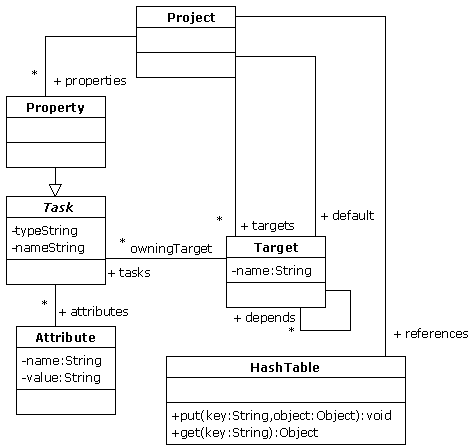
\includegraphics{images/AntCore.png}
	\caption{Simplified ANT object model}
	\label{fig:AntCore}
\end{figure}

\subsection{Concrete Syntax}

In terms of concrete syntax, ANT provides an XML-based syntax. In Listing \ref{lst:ANTExample}, an exemplar ANT project that compiles a set of Java files is illustrated. The project contains one target (\emph{main}) which is also set to be the \emph{default} target. The \emph{main} target contains one \emph{javac} task that specifies attributes such as \emph{srcdir}, \emph{destdir} and \emph{classpath}, which define that the Java compiler will compile a set of Java files contained into the \emph{src} directory into classes that should be placed in the \emph{buiild} directory using \emph{dependencies.jar} as an external library.

\begin{lstlisting}[caption=Compiling Java classes using the javac task, label=lst:ANTExample]
<project default="main">
	<target name="main"/>
	  <javac srcdir="${src}"
	         destdir="${build}"
	         classpath="dependencies.jar"
	         debug="on"
	         source="1.4"/>
	</target>
</project>
\end{lstlisting}

\subsection{Extending ANT}

Binding between the XML tags that describe the tasks and the actual implementations of the tasks is achieved through a light-weight mechanism at two levels. First, the tag (in the example of Listing \ref{lst:ANTExample}, \emph{javac}) is resolved to a Java class that extends the \emph{org.apache.ant.Task} abstract class (in the case of \emph{javac}, the class is \emph{org.apache.tools.ant.taskdefs.Javac}) via a configuration file. Then, the attributes of the tasks (e.g. \emph{srcdir}) are set using the reflective features that Java provides. Finally, the \emph{execute()} method of the task is invoked to perform the actual job.

This lightweight and straightforward way of defining tasks has rendered ANT particularly popular in the Java development community and currently there is a large number of tasks contributed by ANT users \cite{AntExternalTasks}, ranging from invoking tools such as code generators and XSLT processors, to emulating logical control flow structures such as \emph{if} conditions and \emph{while} loops. The AMMA platform \cite{AMMA} also provides integration of model driven engineering tools such as TCS \cite{TCS} and ATL \cite{ATL} with ANT.

ANT also supports more advanced features including nested XML elements and \emph{filesets}, however providing a complete discussion is beyond the scope of this paper. For a definitive guide to ANT readers can refer to \cite{AntBook}.

\section{Integration Challenges}
\label{sec:Workflow.IntegrationChallenges}

A simple approach to extending ANT with support for model management tasks would be to implement one standalone task for each language in Epsilon. However, such an approach demonstrates a number of integration and performance shortcomings which are discussed below. 

Since models are typically serialized in the file system, before a task is executed, the models it needs to access/modify must be parsed and loaded in memory. In the absence of a more elaborate framework, each model management task would have to take responsibility for loading and storing the models it operates on. Also, in most workflows, more than one task operates on the same models sequentially, and needlessly loading/storing the same models many times in the context of the same workflow is an expensive operation both time and memory-wise, particularly as the size of models increases.

Another weakness of this primitive approach is limited inter-task communication. In the absence of a communication framework that allows model management tasks to exchange information with each other, it is often the case that many tasks end up performing the same (potentially expensive) queries on models. By contrast, an inter-task communication framework would enable time and resource intensive calculations to be performed once and their results to be communicated to all interested subsequent tasks.

Having discussed ANT, Epsilon and the challenges their integration poses, the following sections presents the design of a solution that enables developers to invoke model management tasks in the context of ANT workflows. The solution consists of a core framework that addresses the challenges discussed in Section \ref{sec:Workflow.IntegrationChallenges}, a set of specific tasks, each of which implements a distinct model management activity, and a set of tasks that enable developers to initiate and manage transactions on models using the respective facilities provided by the model connectivity layer discussed in Section \ref{sec:EMC.ModelTransactionSupport}. 

\section{Framework Design and Core Tasks}
\label{sec:Workflow.Framework}

The role of the core framework, illustrated in Figure \ref{fig:Core}, is to provide model loading and storing facilities as well as runtime communication facilities to the individual model management tasks that build atop it. This section provides a detailed discussion of the components it consists of.

\begin{landscape}
\begin{figure}
	\centering
		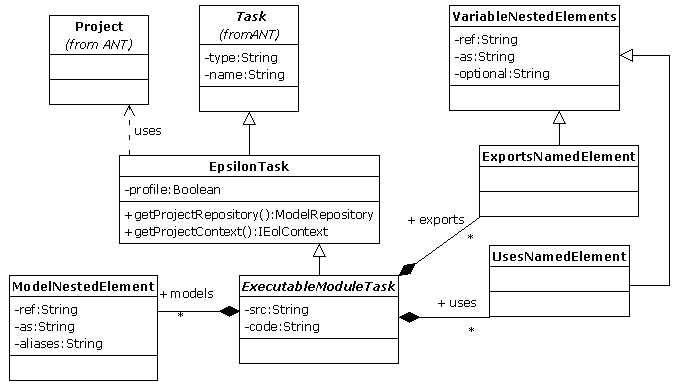
\includegraphics{images/AntEpsilon.png}
	\caption{Core Framework}
	\label{fig:Core}
\end{figure}
\end{landscape}

\begin{figure}
	\centering
		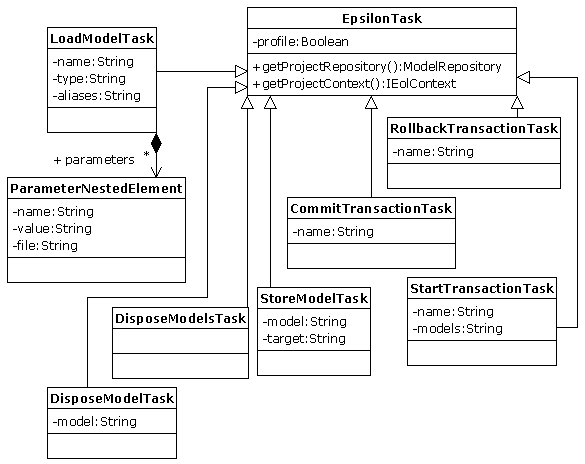
\includegraphics{images/AntEpsilonModels.png}
	\caption{Core Models Framework}
	\label{fig:CoreModels}
\end{figure}

\subsection{The EpsilonTask task}
An ANT task can access the project in which it is contained by invoking the \emph{Task.getProject()} method. To facilitate sharing of arbitrary information between tasks, ANT projects provide two convenience methods, namely \emph{addReference(String key, Object ref)} and \emph{getReference(String key) : Object}. The former is used to add key-value pairs, which are then accessible using the latter from other tasks of the project.

To avoid loading models multiple times and to enable on-the-fly management of models from different Epsilon modules without needing to store and re-load the models after each task, a reference to a project-wide model repository has been added to the current ANT project using the \emph{addReference} method discussed above. In this way, all the subclasses of the abstract \emph{EpsilonTask} can invoke the \emph{getProjectRepository()} method to access the project model repository. 

Also, to support a variable sharing mechanism that enables inter-task communication, the same technique has been employed; a shared context, accessible by all Epsilon tasks via the \emph{getProjectContext()} method, has been added. Through this mechanism, model management tasks can export variables to the project context (e.g. traces or lists containing results of expensive queries) which other tasks can then reuse.

\emph{EpsilonTask} also specifies a \emph{profile} attribute that defines if the execution of the task must be profiled using the profiling features provided by Epsilon. Profiling is a particularly important aspect of workflow execution, especially where model management languages are involved. The main reason is that model management languages tend to provide convenient features which can however be computationally expensive (such as the \emph{allInstances()} EOL built-in feature that returns all the instances of a specific metaclass in the model) and when used more often than really needed, can significantly degrade the overall performance.

%\subsection{Tasks for Loading and Storing Models}

\subsection{Model Loading Tasks}

The \textit{LoadModelTask (epsilon.loadModel)} loads a model from an arbitrary location (e.g. file-system, database) and adds it to the project repository so that subsequent Epsilon tasks can query or modify it. Since Epsilon supports many modelling technologies (e.g. EMF, MDR, XML), the \textit{LoadModelTask} defines only three generic attributes. The \textit{name} attribute specifies the name of the model in the project repository. The \textit{type} attribute specifies the modelling technology with which the model is captured and is used to resolve the technology-specific model loading functionality. Finally, the \textit{aliases} attribute defines a comma-separated list of alternative names by which the model can be accessed in the model repository.

The rest of the information needed to load a model is implementation-specific and is therefore provided through \textit{parameter} nested elements, each one defining a pair of \textit{name}-\textit{value} attributes. As an example, a task for loading an EMF model that has a file-based ECore metamodel is displayed in Listing \ref{lst:LoadModelTask}.

\begin{lstlisting}[float=tbp, basicstyle=\ttfamily\footnotesize, nolol=true, flexiblecolumns=true, caption=Loading an EMF model using the epsilon.loadModel task, label=lst:LoadModelTask, language=XML]
<epsilon.loadModel name="Tree1" type="EMF">
	<parameter name="modelFile" value="TreeInstance.ecore"/>
	<parameter name="metamodelFile" path="Tree.ecore"/>
	<parameter name="isMetamodelFileBased" value="true"/>
	<parameter name="readOnLoad" value="true"/>
</epsilon.loadModel>
\end{lstlisting}%$

\textit{LoadEmfModelTask} is a specialised version of \textit{LoadModelTask} only for EMF models. While the \textit{type} attribute is no longer available, the task still supports the \textit{name} and \textit{aliases} attributes. In addition, some of the values which had to be provided through \textit{parameter} nested elements can now be set using regular attributes, such as \textit{modelFile}, \textit{modelUri}, \textit{metamodelFile} (which implicitly indicates that the metamodel is file-based), \textit{metamodelUri}, \textit{read} (equivalent to \textit{readOnLoad}) and \textit{store} (equivalent to \textit{storeOnDisposal}). Listing~\ref{lst:LoadEmfModelTask} shows the equivalent fragment required to produce the same result as in Listing~\ref{lst:LoadModelTask}.

\begin{lstlisting}[float=tbp, basicstyle=\ttfamily\footnotesize, nolol=true, flexiblecolumns=true, caption=Loading an EMF model using the epsilon.emf.loadModel task, label=lst:LoadEmfModelTask, language=XML]
<epsilon.emf.loadModel name="Tree1"
  modelFile="TreeInstance.ecore"
  metamodelFile="Tree.ecore" />
\end{lstlisting}

\subsection{Model Storing Task}

The \textit{StoreModelTask (epsilon.storeModel)} is used to store a model
residing in the project repository. The \textit{StoreModelTask} defines three
attributes:

\begin{itemize}
\item \textit{name} (required): name of the model to be stored.
\item \textit{targetUri} (optional): URI where the model will be stored (e.g.
  ``file:/path/to/destination'').
\item \textit{target} (optional): file path where the model will be stored (e.g.
  ``file.xmi'').
\end{itemize}

\textit{targetUri} takes precedence over \textit{target}. If neither is defined,
then the model is stored in the location from which it was originally loaded.

\subsection{Model Disposal Tasks}

When a model is no longer required by tasks of the workflow, it can be disposed using the \emph{epsilon.disposeModel} task. The task provides the \emph{model} attribute that defines the name of the model to be disposed. Also, the attribute-less \emph{epsilon.disposeModels} task is provided that disposes all the models in the project model repository. This task is typically invoked when the model management part of the workflow has finished.

The workflow leverages the model-transaction services provided by the model connectivity framework of Epsilon by providing three tasks for managing transactions in the context of workflows.

\subsection{The StartTransaction Task}

The \emph{epsilon.startTransaction} task defines a \emph{name} attribute that identifies the transaction. It also optionally defines a comma-separated list of model names (\emph{models}) that the transaction will manage. If the \emph{models} attribute is not specified, the transaction involves all the models contained in the common project model repository.

\subsection{The CommitTransaction and RollbackTransaction Tasks}

The \emph{epsilon.commitTransaction} and \emph{epsilon.rollbackTransaction} tasks define a \emph{name} attribute through which the transaction to be committed/rolled-back is located in the project's active transactions. If several active transactions with the same name exist the more recent one is selected.

The example of Listing \ref{lst:ANTTransactionsExample} demonstrates an exemplar usage of the \emph{epsilon.startTransaction} and \emph{epsilon.rollbackTransaction} tasks. In this example, two empty models Tree1 and Tree2 are loaded in lines 1,2. Then, the EOL task of line \ref{line:initialQuery} queries the models and prints the number of instances of the \emph{Tree} metaclass in each one of them (which is 0 for both). Then, in line \ref{line:transactionStart}, a transaction named T1 is started on model Tree1. The EOL task of line \ref{line:newInstances}, creates a new instance of Tree in both Tree1 and Tree2 and prints the number of instances of Tree in the two models (which is 1 for both models). Then, in line \ref{line:transactionRollback}, the T1 transaction is rolled-back and any changes done in its context to model Tree1 (but not Tree2) are undone. Therefore, the EOL task of line \ref{line:finalQuery}, which prints the number of instances of Tree in both models, prints 0 for Tree1 but 1 for Tree2.

\begin{lstlisting}[caption=Exemplar usage of the \emph{epsilon.startTransaction} and \emph{epsilon.rollbackTransaction} tasks, label=lst:ANTTransactionsExample, language=XML]
<epsilon.loadModel name="Tree1" type="EMF">...</epsilon.loadModel>
<epsilon.loadModel name="Tree2" type="EMF">...</epsilon.loadModel>

<epsilon.eol>/*@\label{line:initialQuery}@*/
	<![CDATA[
	Tree1!Tree.allInstances.size().println(); // prints 0 
	Tree2!Tree.allInstances.size().println(); // prints 0
	]]>
	<model ref="Tree1"/>
	<model ref="Tree2"/>
</epsilon.eol>

<epsilon.startTransaction name="T1" models="Tree1"/> /*@\label{line:transactionStart}@*/

<epsilon.eol> /*@\label{line:newInstances}@*/
	<![CDATA[
	var t1 : new Tree1!Tree; 
	Tree1!Tree.allInstances.size().println(); // prints 1
	var t2 : new Tree2!Tree;
	Tree2!Tree.allInstances.size().println(); // prints 1
	]]>
	<model ref="Tree1"/>
	<model ref="Tree2"/>
</epsilon.eol>

<epsilon.rollbackTransaction name="T1"/> /*@\label{line:transactionRollback}@*/

<epsilon.eol>/*@\label{line:finalQuery}@*/
	<![CDATA[
	Tree1!Tree.allInstances.size().println(); // prints 0 
	Tree2!Tree.allInstances.size().println(); // prints 1 
	]]>
	<model ref="Tree1"/>
	<model ref="Tree2"/>
</epsilon.eol>
\end{lstlisting}

%\subsection{Model Management Tasks}

\subsection{The Abstract Executable Module Task}
\label{sec:ExecutableModuleTask}

This task is the base of all the model management tasks presented in Section \ref{sec:Workflow.ModelManagementTasks}. Its aim is to encapsulate the commonalities of Epsilon tasks in order to reduce duplication among them. As already discussed, in Epsilon, specifications of model management tasks are organized in executable modules. While modules can be stored anywhere, in the case of the workflow it is assumed that they are either stored as separate files in the file-system or they are provided inline within the worfklow. Thus, this abstract task defines an \textit{src} attribute that specifies the path of the source file in which the Epsilon module is stored, but also supports inline specification of the source of the module. The two alternatives are demonstrated in Listings \ref{lst:External} and \ref{lst:Inline} respectively.

\begin{lstlisting}[basicstyle=\ttfamily\footnotesize, flexiblecolumns=true, numbers=none, nolol=true, caption=External Module Specification, label=lst:External, numbers=left, language=XML, tabsize=2]
<project default="main">
	<target name="main">
		<epsilon.eol src="HelloWorld.eol"/>
	</target>
</project>
\end{lstlisting}

\begin{lstlisting}[basicstyle=\ttfamily\footnotesize, flexiblecolumns=true, numbers=none, nolol=true, caption=Inline Module Specification, label=lst:Inline, numbers=left, language=XML, tabsize=2]
<project default="main">
	<target name="main">
		<epsilon.eol>
			<![CDATA[
				'Hello world'.println();
			]]>
		</epsilon.eol>
	</target>
</project>
\end{lstlisting}


The task also defines the following nested elements:

\paragraph{0..n $model$ nested elements}

Through the \emph{model} nested elements, each task can define which of the models, loaded in the project repository it needs to access. Each \emph{model} element defines three attributes. The \emph{ref} attribute specifies the name of the model that the task needs to access, the \emph{as} attribute defines the name by which the model will be accessible in the context of the task, and the \emph{aliases} defines a comma-delimited sequence of aliases for the model in the context of the task.

\paragraph{0..n $parameter$ nested elements}

The \emph{parameter} nested elements enable users to communicate String parameters to tasks. Each \emph{parameter} element defines a \emph{name} and a \emph{value} attribute. Before executing the module, each \emph{parameter} element is transformed into a String variable with the respective name and value which is then made accessible to the module.

\paragraph{0..n $exports$ nested elements}

To facilitate low-level integration between different Epsilon tasks, each task can export a number of variables to the project context, so that subsequent tasks can access them later. Each \emph{export} nested element defines the three attributes. The \emph{ref} attribute specifies the name of the variable to be exported, the \emph{as} string attribute defines the name by which the variable is stored in the project context and the \emph{optional} boolean attribute specifies whether the variable is mandatory. If \emph{optional} is set to \emph{false} and the module does not specify such a variable, an ANT \emph{BuildException} is raised.

\paragraph{0..n $uses$ nested elements}

The \emph{uses} nested elements enable tasks to import variables exported by previous Epsilon tasks. Each use element supports three attributes. The \emph{ref} attribute specifies the name of the variable to be used. If there is no variable with this name in the project context, the ANT project properties are queried. This enables Epsilon modules to access ANT parameters (e.g. provided using command-line arguments). The \emph{as} attribute specifies the name by which the variable is accessible in the context of the task. Finally, the \emph{optional} boolean paramter specifies if the variable must exist in the project context.

To better illustrate the runtime communication mechanism, a minimal example is provided in Listings \ref{lst:Exporter} - \ref{lst:ExporterUserWorkflow}. In Listing \ref{lst:Exporter}, \emph{Exporter.eol} defines a String variable named \emph{x} and assigns a value to it. The workflow of Listing \ref{lst:ExporterUserWorkflow} specifies that after executing \emph{Exporter.eol}, it must export a variable named \emph{x} with the new name \emph{y} to the project context. Finally, it defines that before executing \emph{User.eol} (Listing \ref{lst:User}), it must query the project context for a variable named \emph{y} and in case this is available, add the variable to the module's context and then execute it. Thus, the result of executing the workflow is \emph{Some String} printed in the output console.

\begin{lstlisting}[basicstyle=\ttfamily\footnotesize, nolol=true, flexiblecolumns=true, caption=Source code of the Exporter.eol module, label=lst:Exporter, language=EOL]
var x : String := 'Some string';
\end{lstlisting}

\begin{lstlisting}[basicstyle=\ttfamily\footnotesize, nolol=true, flexiblecolumns=true, caption=Source code of the User.eol module, label=lst:User, language=EOL]
z.println();
\end{lstlisting}

\begin{lstlisting}[basicstyle=\ttfamily\footnotesize, nolol=true, flexiblecolumns=true, caption=ANT Workflow connecting modules  \ref{lst:Exporter} and \ref{lst:User} using the epsilon.eol task, label=lst:ExporterUserWorkflow , language=XML]
<epsilon.eol src="Exporter.eol">
	<exports ref="x" as="y"/>
</epsilon.eol>

<epsilon.eol src="User.eol">
	<uses ref="y" as="z"/>
</epsilon.eol>
\end{lstlisting}

\section{Model Management Tasks}
\label{sec:Workflow.ModelManagementTasks}
  
Having discussed the core framework, this section presents the model management tasks that have been implemented atop it, using languages of the Epsilon platform.

\begin{figure}[ht!]
	\centering
		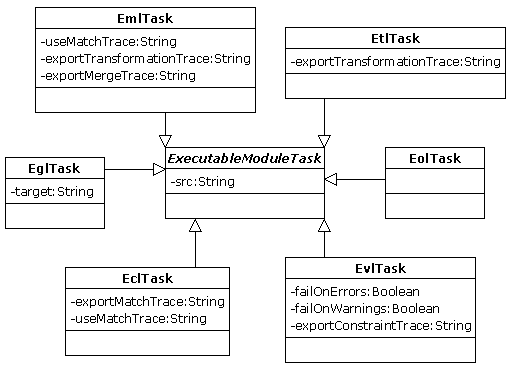
\includegraphics{images/Tasks.png}
	\caption{Model Management Tasks}
	\label{fig:Tasks}
\end{figure}

\subsection{Generic Model Management Task}
\label{sec:EolTask}

The \emph{epsilon.eol} task executes an EOL module, defined using the \emph{src} attribute on the models that are specified using the \emph{model} nested elements.
\subsection{Model Validation Task}
\label{sec:EvlTask}

The \emph{epsilon.evl} task executes an EVL module, defined using the \emph{src} attribute on the models that are specified using the \emph{model} nested elements. In addition to the attributes defined by the ExecutableModuleTask, this task also provides the following attributes:

\begin{itemize}
	\item \emph{failOnErrors} : Errors are the results of unsatisfied constraints. Setting the value of this attribute to \emph{true} (default is \emph{false}) causes a \emph{BuildException} to be raised if one or more errors are identified during the validation process.
	\item \emph{failOnWarnings} : Similarly to errors, warnings are the results of unsatisfied critiques. Setting the value of this atrribute to \emph{true} (default is also \emph{false}) causes a \emph{BuildException} to be raised if one or more warnings are identified during the validation process.
	\item \emph{exportConstraintTrace} : This attribute enables developers to export the internal constraint trace constructed during model validation to the project context so that it can be later accessed by other tasks - which could for example attempt to automatically repair the identified inconsistencies. 
\end{itemize}

\subsection{Model-to-Model Transformation Task}

The \emph{epsilon.etl} task executes an ETL module, defined using the \emph{src} attribute to transform between the models that are specified using the \emph{model} nested elements. In addition to the attributes defined by the ExecutableModuleTask, this task also provides the \emph{exportTransformationTrace} attribute that enables the developer to export the internal transformation trace to the project context. In this way this trace can be reused by subsequent tasks; for example another task can serialize it in the form of a separate traceability model.

\subsection{Model Comparison Task}

The \emph{epsilon.ecl} task executes an ECL module, defined using the \emph{src} attribute to establish matches between elements of the models that are specified using the \emph{model} nested elements. In addition to the attributes defined by the ExecutableModuleTask, this task also provides the \emph{exportMatchTrace} attribute that enables users to export the match-trace calculated during the comparison to the project context so that subsequent tasks can reuse it. For example, as discussed in the sequel, an EML model merging task can use it as a means of identifying correspondences on which to perform merging. In another example, the match-trace can be stored by a subsequent EOL task in the form of an stand-alone weaving model.


\subsection{Model Merging Task}

The \emph{epsilon.eml} task executes an EML module, defined using the \emph{src} attribute on the models that are specified using the \emph{model} nested elements. In addition to the attributes defined by the ExecutableModuleTask, this task also provides the following attributes:

\begin{itemize}
	\item \emph{useMatchTrace} : As discussed in \ref{sec:EML}, to merge a set of models, an EML module needs an established match-trace between elements of the models. The \emph{useMatchTrace} attribute enables the EML task to use a match-trace exported by a preceeding ECL task (using its \emph{exportMatchTrace} attribute).
	\item \emph{exportMergeTrace, exportTransformationTrace} : Similarly to ETL, through these attributes an EML task can export the internal traces calculated during merging for subsequent tasks to use.
\end{itemize}

%!TEX root = ../EpsilonBook.tex

\subsection{Model-to-Text Transformation Task}
\label{sec:EglTask}
To support model to text transformations, \textit{EglTask (epsilon.egl)} task is provided that executes an Epsilon Generation Language (EGL) module\footnote{As discussed in Section \ref{sec:EGL} EGL has been built atop Epsilon with a minimal contribution of the author}. In addition to the attributes defined by \textit{ExecutableModuleTask}, \textit{EglTask} also defines the following attributes:

\begin{itemize}
	\item \textit{target} : Defines a file in which all of the generated text will be stored.
	\item \textit{templateFactoryType} : Defines the Java class that will be instantiated to provide a \emph{TemplateFactory} for the EGL program. The specified class must be on the classpath and must subtype \emph{EglTemplateFactory}. See Section~\ref{sec:custom_co-ordination} for more information.
\end{itemize}

\emph{EglTask} may nest any number of \emph{formatter} elements. The \emph{formatter} nested element has the following attributes:

\begin{itemize}
	\item \textit{implementation} (required) : Defines the Java class that will be instantiated to provide a \emph{Formatter} for the EGL program. The specified class must be on the classpath and must subtype \emph{Formatter}. See Section~\ref{sec:custom_formatter} for more information.
\end{itemize}

%!TEX root = ./EpsilonBook.tex

\chapter{Epsilon Flock for Model Migration}
\label{sec:Flock}

The aim of Epsilon Flock is to contribute \emph{model migration} capabilities to Epsilon. Model migration is the process of updating models in response to metamodel changes. This section discusses the motivation for implementing Flock, introduces its syntax and execution semantics, and demonstrates the use of Flock with an example.
Flock can be used to update models to a new version of their metamodel, or even to move from one modelling technology to another (e.g., from XML to EMF).

\section{Background and Motivation}
\label{sec:flock_background}
Model migration involves updating a model in response to changes to the metamodel. Typically, metamodel evolution is accomplished incrementally: changes are made to part of the metamodel and hence model migration typically involves updating only a small proportion of a model's elements \cite{sprinkle03thesis,herrmannsdoerfer08automatability}. Effectively then, model migration is a model-to-model transformation in which the source and target metamodels are similar but not the same. However, as discussed below, model-to-model transformation languages are often cumbersome for specifying model migration.

To illustrate the challenges of model migration, we use the example of metamodel evolution in Figure~\ref{fig:po_mms}. In Figure~\ref{fig:original_po_mm}, a \texttt{Co\-mp\-on\-e\-nt} comprises other \texttt{Co\-mp\-on\-e\-nt}s, \texttt{Co\-nn\-ec\-t\-or}s and \texttt{Po\-rt}s. A \texttt{Co\-nn\-ec\-t\-or} joins two \texttt{Po\-rt}s. \texttt{Co\-nn\-ec\-t\-or}s are unidirectional, and hence define \texttt{to} and \texttt{fr\-om} references to \texttt{Po\-rt}. The original metamodel allows a \texttt{Co\-nn\-ec\-t\-or} to start and end at the same \texttt{Po\-rt}, and the metamodel was evolved to prevent this, as shown in Figure~\ref{fig:evolved_po_mm}. \texttt{Po\-rt} was made abstract, and split into two subtypes, \texttt{In\-p\-utPo\-rt} and \texttt{Ou\-t\-putPo\-rt}. The references between \texttt{Co\-nn\-ec\-t\-or} and (the subtypes of) \texttt{Po\-rt} were renamed for consistency with the names of the subtypes.

Some models that conform to the original metamodel do not conform to the evolved metamodel. Specifically, models might not conform to the evolved metamodel because:

\begin{enumerate}
	\item They contain instances of \texttt{Port}, which is an abstract class in the evolved metamodel.
	\item They contain instances of \texttt{Connector} that specify values for the features \texttt{to} and \texttt{from}, which are not defined for the \texttt{Connector} type in the evolved metamodel.
	\item They contain instances of \texttt{Connector} that do not specify a value for the \texttt{in} and \texttt{out} features, which are mandatory for the \texttt{Connector} type in the evolved metamodel.
\end{enumerate}

Model migration can be achieved with a general-purpose model-to-model transformation using a language such as ETL (Chapter~\ref{sec:ETL}). However, this typically involves writing a large amount of repetitive and redundant code \cite{rose12flock}. Flock reduces the amount of repetitive and redundant code needed to specify model migration by automatically copying from the original to the migrated model all of the model elements that conform to the evolved metamodel as described below.


\begin{landscape}
\begin{figure}[htbp]
	\centering
	\subbottom[Original metamodel.]
	{
	    \label{fig:original_po_mm}
	    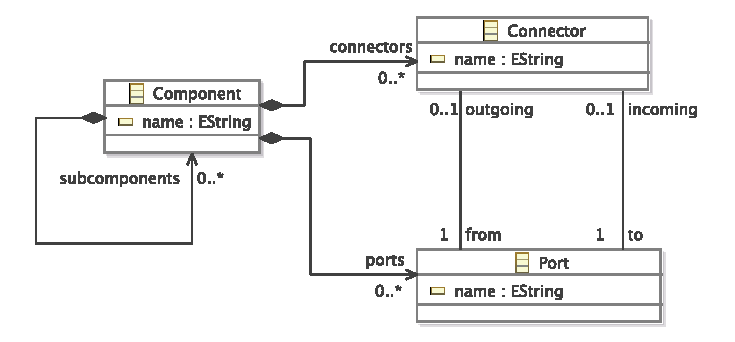
\includegraphics{images/FlockPOExampleOriginal.pdf}
	}
	\subbottom[Evolved metamodel.]
	{
	    \label{fig:evolved_po_mm}
	    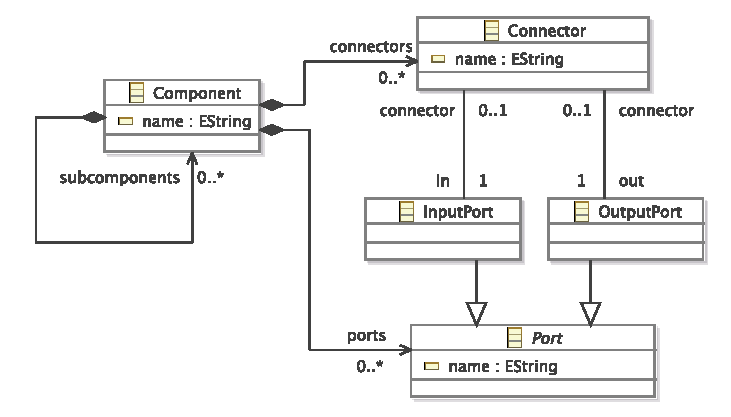
\includegraphics{images/FlockPOExampleEvolved.pdf}
	}
	\caption{Process-oriented metamodel evolution.}
\label{fig:po_mms}
\end{figure}
\end{landscape}

\begin{landscape}
\begin{figure}
	\centering
		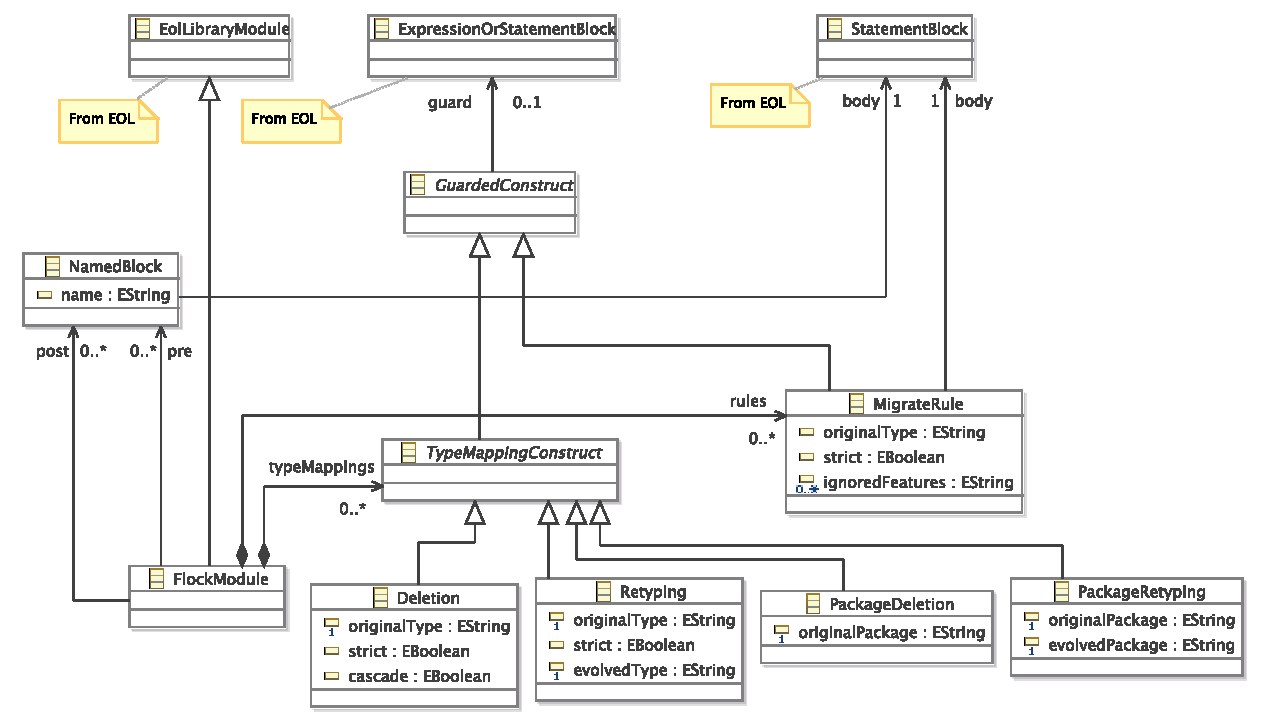
\includegraphics{images/FlockAbstractSyntax.pdf}
	\caption{The Abstract Syntax of Flock}
	\label{fig:flock_abstract_syntax}
\end{figure}
\end{landscape}


\section{Abstract Syntax}

As illustrated by Figure~\ref{fig:flock_abstract_syntax}, Flock migration strategies are organised into individual modules (\texttt{Flo\-ckMo\-du\-le}). Flock modules inherit from EOL language constructs for specifying user-defined operations and for importing other (EOL and Flock) modules. Flock modules comprise any number of type mappings (\texttt{Ty\-peMa\-pp\-i\-ng}) and rules (\texttt{Ru\-le}). Type mappings operate on metamodel types (\texttt{Rety\-pi\-ng} and \texttt{De\-le\-ti\-on}) or on metamodel packages (\texttt{Pa\-ck\-a\-geRety\-pi\-ng} and \texttt{Pa\-ck\-a\-geDe\-le\-ti\-on}. Type mappings are applied to a type in the original metamodel (\texttt{or\-ig\-in\-alTy\-pe}) or to a package in the original metamodel (\texttt{or\-ig\-in\-alPa\-ck\-a\-ge}) . Additionally, \texttt{Rety\-pi\-ng}s apply to an evolved metamodel type (\texttt{ev\-ol\-vedTy\-pe}) or package (\texttt{ev\-ol\-vedPa\-ck\-a\-ge}). Each rule has an original metamodel type (\texttt{or\-ig\-in\-alTy\-pe}), a \texttt{bo\-dy} comprising a block of EOL statements, and zero or more \texttt{ig\-no\-r\-edFe\-at\-ur\-es}. Type mappings and rules can optionally specify a \texttt{gu\-ard}, which is either an EOL statement or a block of EOL statements. Type mappings that operate on metamodel types and rules can be marked as \texttt{str\-ict}.

\section{Concrete Syntax}

Listing \ref{lst:FlockConcreteSyntax} demonstrates the concrete syntax of the Flock language constructs. All of the constructs begin with keyword(s) (\texttt{retype}, \texttt{retype package} \texttt{delete}, \texttt{delete package} or \texttt{migrate}), followed by the original metamodel type or package. Additionally, type mappings that operate on metamodel types and rules can be annotated with the \texttt{strict} modifier. All constructs can have guards, which are specified using the \texttt{when} keyword.

Migrate rules can specify a list of features that conservative copy will ignore (\texttt{ignoring}), and a \texttt{body} containing a sequence of at least one EOL statement. Note that a migrate rule must have a list of ignored features, or a body, or both.

\begin{lstlisting}[caption={Concrete syntax of Flock retypings, deletions and migrate rules}, label=lst:FlockConcreteSyntax, language=Flock]
(@strict)?
retype <originalType> to <evolvedType>
(when (:<eolExpression>)|({<eolStatement>+}))?

retype package <originalPackage> to <evolvedPackage>
(when (:<eolExpression>)|({<eolStatement>+}))?

(@strict)?
delete <originalType>
(when (:<eolExpression>)|({<eolStatement>+}))?

delete package <originalPackage>
(when (:<eolExpression>)|({<eolStatement>+}))?

(@strict)?
migrate <originalType>
(ignoring <featureList>)?
(when (:<eolExpression>)|({<eolStatement>+}))? {
	<eolStatement>+
}
\end{lstlisting}



\section{Execution Semantics}
The execution semantics of a Flock module are now described. Note that the Epsilon Model Connectivity (EMC) layer (Chapter~\ref{sec:Design.EMC}), which Flock uses to access and manipulate models supports a range of modelling technologies, and identifies types by name. Consequently, the term \emph{type} is used to mean ``the name of an element of a metamodel'' in the following discussion. For example, \texttt{Co\-mp\-on\-e\-nt}, \texttt{Co\-nn\-ec\-t\-or} and \texttt{In\-p\-utPo\-rt} are three of the types defined in Figure~\ref{fig:evolved_po_mm}.

Execution of a Flock module occurs in four phases. Firstly, type mapping constructs (retypings and deletions) are processed to identify the way in which original and evolved metamodel types are to be related. Secondly, migrate rules are inspected to build sets of ignored properties. Thirdly, the information determined in steps 1 and 2 is used as input a copying algorithm, which creates an (equivalent) element in the migrated model for each element of the original model, and copies values from original to equivalent model elements. Finally, migrate rules are executed on each pair of original and (equivalent) migrated model elements. In all phases, language constructs are executed only when they are \emph{applicable}.

The \emph{applicability} of the Flock language constructs (retyping, deletion or migrate rule) is determined from their type and guard. For a language construct $c$ to be applicable to an original model element $o$, $o$ must instantiate either the original type of $c$ or one of the subtypes of the original type of $c$; and $o$ must satisfy the guard of $c$. For language constructs that have been annotated as strict, type-checking is more restrictive: $o$ must instantiate the original type of $c$ (and not one its subtypes). In other words, the applicability of strict constructs is determined with EOL's \texttt{isTypeOf} operation and the applicability of non-strict constructs is determined with EOL's \texttt{isKindOf} operation (Table~\ref{tab:AnyOperations}). For language constructs that operate on packages (i.e. package retyping and package deletions), type-checking is less restrictive: $o$ must be contained in a package with the same name as the original package of $c$.

The first three phases of execution implement a copying algorithm which has been termed conservative copy and is discussed thoroughly elsewhere \cite{rose12flock}. Essentially, conservative copy will do the following for each element of the original model, $o$:

\begin{enumerate}
	\item \textbf{Do nothing} when $o$ instantiates a type that cannot be instantiated in the evolved metamodel (e.g., because the type of $o$ is now abstract or no longer exists). Example: instances of \texttt{Port} in Figure~\ref{fig:po_mms} are not copied because \texttt{Port} has become abstract.
	\item \textbf{Fully copy} $o$ to produce $m$ in the migrated model when $o$ instantiate a type that has not been at all affected by metamodel evolution. Example: instances of \texttt{Component} in Figure~\ref{fig:po_mms} are fully copied because neither \texttt{Component} nor any of its features have been changed.
	\item \textbf{Partially copy} $o$ to produce $m$ in the migrated model when $o$ instantiates a type with one or more features that have been affected by metamodel evolution. Example: instances of \texttt{Connector} in Figure~\ref{fig:po_mms} are partially copied because the \texttt{from} and \texttt{to} features have been renamed. Note that in a partial copy only the features that have not been affected by metamodel evolution are copied (e.g., the \texttt{name}s of \texttt{Connector}s).
\end{enumerate}

In the fourth phase of execution, migrate rules are applied. These rules specify the problem-specific migration logic and might, for example, create migrated model elements for original model elements that were skipped or partially copied by the copying algorithm described above. The Flock engine makes available two variables (\texttt{or\-ig\-in\-al} and \texttt{mi\-gr\-at\-ed}) for use in the body of any migration rule. These variables are used to refer to the particular elements of the original and migrated models to which the rule is currently being applied. In addition, Flock defines an \texttt{equivalent()} operation that can be called on any original model element and returns the equivalent migrated model element (or \texttt{null}). The \texttt{equivalent()} operation is used to access elements of the migrated model that cannot be accessed via the \texttt{migrated} variable due to metamodel evolution. Flock rules often contain statements of the form: \texttt{original.x.equivalent()} where \texttt{x} is a feature that has been removed from the evolved metamodel.

Finally, we should consider the order in which Flock schedules language constructs: a construct that appears earlier (higher) in the source file has priority. This is important because only one type mapping (retypings and deletions) is applied per original model element, and because this implies that migrate rules are applied from top-to-bottom. This ordering is consistent with the other languages of the Epsilon platform.

\begin{figure}[tbp]
	\begin{framed}
		\footnotesize
		\begin{itemize}
			\item For every instance, p, of \texttt{Port} in the original model: 
			\subitem $-$ If there exists in the original model a \texttt{Connector}, c, that specifies p as the value for its \texttt{from} feature:
			\subsubitem $-$ Create a new instance, i, of \texttt{InputPort} in the migrated model.
			\subsubitem $-$ Set c as the \texttt{connector} of i.
			\subsubitem $-$ Add c to the \texttt{ports} reference of the \texttt{Component} that contains c.
	
			\subitem $-$ If there exists in the original model a \texttt{Connector}, c, that specifies p as the value for its \texttt{to} feature:
			\subsubitem $-$ Create a new instance of \texttt{OutputPort} in the migrated model.
			\subsubitem $-$ Set c as the \texttt{connector} of i.
			\subsubitem $-$ Add c to the \texttt{ports} reference of the \texttt{Component} that contains c.

			\item And nothing else changes.
		\end{itemize}
	\end{framed}
	\caption{Model migration strategy in pseudo code for the metamodel evolution in Figure~\ref{fig:po_mms}.}
	\label{fig:po_migration_strategy}
\end{figure}

\begin{lstlisting}[caption=Flock migration strategy for the process-oriented metamodel evolution in Figure~\ref{fig:po_mms}, label=lst:flock, language=Flock]
delete Port when: not (original.isInput() xor original.isOutput())

retype Port to InputPort  when: original.isInput()
retype Port to OutputPort when: original.isOutput()

migrate Connector {
	migrated.`in` = original.from.equivalent();
	migrated.out = original.`to`.equivalent();
}

operation Original!Port isInput() : Boolean {
	return Original!Connector.all.exists(c|c.from == self);
}

operation Original!Port isOutput() : Boolean {
	return Original!Connector.all.exists(c|c.`to` == self);
}
\end{lstlisting}

\section{Example}
Flock is now demonstrated using the example of model migration introduced in Section~\ref{sec:flock_background}. Recall that the metamodel evolution in Figure~\ref{fig:po_mms} involves splitting the \texttt{Po\-rt} type to form the \texttt{In\-p\-utPo\-rt} and \texttt{Ou\-tp\-utPo\-rt} types. Figure~\ref{fig:po_migration_strategy} provides a high-level design for migrating models from the original to the evolved metamodel in Figure~\ref{fig:po_mms}.


The Flock migration strategy that implements this design is shown\footnote{Note that \texttt{in} and \texttt{to} are reserved words in EOL, and hence backticks are used to refer to the metamodel features \texttt{in} and \texttt{to} on lines 7, 8 and 16 of Listing~\ref{lst:flock}.} in Listing~\ref{lst:flock}. Three type mappings constructs (on lines 1-4) are used to control the way in which instances of \texttt{Po\-rt} are migrated. For example, line 3 specifies that instances of \texttt{Po\-rt} that are referenced via the \texttt{fr\-om} feature of a \texttt{Co\-nn\-ec\-t\-or} are retyped, becoming \texttt{In\-pu\-tPo\-rt}s. Instances of \texttt{Co\-nn\-ec\-t\-or} are migrated using the rule on lines 6-9, which specifies the way in which the \texttt{fr\-om} and \texttt{to} features have evolved to form the \texttt{in} and \texttt{out} features.

Note that metamodel elements that have not been affected by the metamodel evolution, such as \texttt{Co\-mp\-on\-e\-nt}s, are migrated automatically. Explicit copying code would be needed to achieve this with a general purpose model-to-model transformation language.

\section{Limitations and Scope}
Although Flock has been shown to much more concise than general purpose model-to-model transformation languages for specifying model migration, Flock does not provide some of the features commonly available in general-purpose model-to-model transformation language. This section discusses the limitations of Flock and its intended scope with respect to other tools for model migration.

\subsection{Limitations}
Firstly, Flock does not support rule inheritance, and re-use of migration logic is instead achieved by exploiting the inheritance hierarchy of the original metamodel. The form of re-use provided by Flock is less general than rule-inheritance, but has proved sufficient for existing use-cases.

Secondly, Flock does not provide language constructs for controlling the order in which rules are scheduled (other than the ordering of the rules in the program file). ATL, for example, includes constructs that allow users to specify that rules are scheduled explicitly (lazy rules) or in a memoised manner (unique rules). We anticipate that scheduling constructs might be necessary for larger migration strategies, but have not yet encountered situations in which they have been required.

Thirdly, Flock is tailored for applying migration to a single original and a single migrated model. Although further models can be accessed by a Flock migration strategy, they cannot be used as the source or target of the conservative copy algorithm. By contrast, some general-purpose model transformation languages can access and manipulate any number of models.

Finally, Flock has been tailored to the model migration problem. In other words, we believe that Flock is well-suited to specifying model transformations between two metamodels that are very similar. For metamodel evolution in which the original metamodel undergoes significant and large-scale revision, a general-purpose transformation might be more suitable than Flock for specifying model migration.

\subsection{Scope}
Flock is typically used as a manual specification approach in which model migration strategies are written by hand. As such, we believe that Flock provides a flexible and concise way to specify migration, and is a foundation for further tools that seek to automate the metamodel evolution and model migration processes. There are approaches to model migration that encompass both the metamodel evolution and model migration processes, seeking to automatically derive model migration strategies (e.g., Edapt \url{http://www.eclipse.org/edapt/}). These approaches provide more automation but at the cost of flexibility: for example, you might be restricted to using a tool-specific editor to perform model migration, or to using only EMF.


\section{Further Reading}
Further examples of applying Flock include migration of UML activity diagrams (at Transformation Tool Contest 2010 workshop\footnote{\url{http://planet-mde.org/ttc2010/}}), and migration of UML class diagrams, GMF models, and a domain-specific modelling language for NNTP newsgroups in Rose's doctoral thesis \cite{rose11thesis}.

A more thorough discussion of the design decisions and execution semantics of Flock can be found in a SoSyM journal article \cite{rose12flock}. Flock has been compared with other model migration tools and languages in a MoDELS paper \cite{rose10comparison}. 
\subsection{Pattern Matching Task}

The \emph{epsilon.epl} task executes an EPL module, defined using the \emph{src} attribute to perform pattern matching on the models that are specified using the \emph{model} nested elements. In addition to the attributes defined by the ExecutableModuleTask, this task also provides the following attributes.

\begin{itemize}
  \item \emph{repeatWhileMatches}: A boolean specifying whether the pattern matching process should continue to execute for as long as matches are found.
  \item \emph{maxLoops}: An integer specifying the maximum number of pattern matching iterations.
  \item \emph{exportAs}: The name under which the computed pattern match model should be made available to other Epsilon tasks of the workflow.
\end{itemize}


\section{Miscellaneous Tasks}

\subsection{Java Class Static Method Execution Task}

The \emph{epsilon.java.executeStaticMethod} task executes a parameter-less static method, defined using the \emph{method} attribute, of a Java class, defined using the \emph{javaClass} attribute. This task can be useful for setting up the infrastructure of Xtext-based languages.

\subsection{Adding a new Model Management Task}
\label{sec:Workflow.NewModelManagementTask}

As discussed in Section \ref{sec:Design.ImplementingANewLanguage}, additional task-specific languages are likely to be needed in the future for tasks that are not effectively supported by existing task-specific languages. In addition to designing and implementing the syntax and execution semantics of a new language, it is also important to provide integration with the workflow -- if the nature of the language permits execution within a workflow. As a counter-example, no workflow task has been provided for EWL since its execution semantics is predominately user-driven and as such, it makes little sense to execute EWL in the context of an automated workflow.

To implement support for a new task-specific language to the workflow, a new extension of the abstract \emph{ExecutableModuleTask} needs to be provided (similarly to what has been done for existing task-specific languages). By extending \emph{ExecutableModuleTask}, the task is automatically provided with access to the essential features of the workflow such as the shared model repository, and runtime context. Additional configuration options for the task need to specified as new ANT \emph{attributes} and/or \emph{nested elements}, similarly to what has been done for the tasks presented in Sections \ref{sec:EolTask}--\ref{sec:EglTask}.

\section{Chapter Summary}

This chapter has presented the detailed design of an ANT-based framework for integrating and orchestrating mainstream software development tasks with model management tasks implemented using model management languages in Epsilon. In Section \ref{sec:Workflow.Framework}, the core framework that provides features such centralized model loading/storing facilities, a shared model repository and a mechanism through which individual tasks can communicate at runtime has been illustrated. Then, Section \ref{sec:Workflow.ModelManagementTasks} has provided a discussion on the integration of the task specific languages with the framework and also provided guidance for adding support for additional languages that are likely to be developed in the future atop Epsilon.